% Build here: pdflatex -interaction=nonstopmode -halt-on-error endterm_report.tex (twice).
% Figures are clipped directly from the supplied paper at the repository root.
\pdfminorversion=5
\pdfobjcompresslevel=0
\documentclass[10pt,twocolumn]{article}
\usepackage[letterpaper,margin=0.68in,columnsep=0.25in]{geometry}
\usepackage[T1]{fontenc}
\usepackage{mathptmx,microtype,amsmath,booktabs,graphicx,caption,titlesec,flushend,needspace}
\usepackage[hidelinks]{hyperref}
\titleformat{\section}{\normalsize\bfseries}{\thesection.}{0.45em}{}
\titlespacing*{\section}{0pt}{8pt}{4pt}
\captionsetup{font=small,labelfont=bf,skip=4pt}
\setlength{\parindent}{1em}
\setlength{\parskip}{1pt}
\setlength{\textfloatsep}{10pt}
\setlength{\intextsep}{9pt}
\raggedbottom
\newcommand{\lookup}{\textsc{Lookup}}
\newcommand{\expand}{\textsc{Expand}}
\newcommand{\code}[1]{{\small\texttt{#1}}}
\begin{document}
\twocolumn[\begin{center}
{\LARGE\bfseries Diamond-Hardened Hash Joins in PostgreSQL\par}
\vspace{5pt}
{\normalsize CS631 End-Term Report: Planning, Cost Models, and Evaluation\par}
\vspace{6pt}
{\small
\begin{tabular}{@{}c@{\hspace{1.3em}}c@{\hspace{1.3em}}c@{\hspace{1.3em}}c@{}}
Harshit Raj & Sumedh SS & Kabir S Prakash & Harshul Suthar\\
23B0950 & 23B1079 & 23B1036 & 23B0968
\end{tabular}\par}
\vspace{7pt}
\end{center}]

\noindent\textbf{Abstract.}
The midterm established a working Lookup--Expand executor that avoided large
intermediate results on a synthetic microbenchmark (200.99$\times$ at $N=1{,}000$,
669.27$\times$ at $N=5{,}000$). This report covers what we built after midterm:
(i)~independent Lookup and Expand executor nodes with a sound ownership contract,
(ii)~an automatic GYO-based acyclic planner that adds Diamond candidates after
standard join search, (iii)~three selectable Expand cost models ending in a
blow-up-robust strategy, and (iv)~evaluation against TPC-H SF1, JOB, and
STATS-CEB. Diamond is correctly not selected on TPC-H and JOB, confirming the
paper's expectation that gains come from skewed multi-join data with selective
late filters. On STATS-CEB, the planner automatically selects Diamond on
4 of 146 queries; Q8 runs 2.19$\times$ faster.

\section{Recap: the problem and the approach}
A hash join builds a table on one input and probes it with the other, emitting
every matching pair immediately. If a later join rejects most of those pairs,
the database wastes time generating a large intermediate that it then discards.
The midterm described this diamond problem and showed how splitting each join
probe into a \lookup{} (find the first match, save its position) and an
\expand{} (enumerate remaining matches later) lets the optimizer push cheap
filters before expensive enumeration.

By the time of this report, all four main implementation phases are complete
in the \code{diamond-pg-cloud} branch of our PostgreSQL~20devel fork.

\section{Independent executor nodes}

The midterm's Phase~2 proved the \lookup{}--\expand{} idea inside a single
HashJoin node, using a borrowed first-match cursor with an immediate expand.
Phase~3 makes the split real: Lookup and Expand are separate PostgreSQL plan
and state nodes, letting the optimizer freely insert other operators between
them.

\paragraph{Lookup node.}
Lookup inherits from \code{HashJoin}/\code{HashJoinState}. Its hash table is
built normally. For each outer probe tuple it calls the existing hash scanner
once, checks equality, and stops at the first match. It copies the probe into
an owned \code{MinimalTuple} (child slots change on the next pull) and records
the first match and its hash-table position in an immutable
\code{DiamondDeferredMatch} descriptor. It appends that descriptor to a sidecar
list that travels with the surviving partial tuple to the next join.

\paragraph{Expand node.}
Expand holds a saved owner reference and a generation counter. On each
demand-pull call it validates the owner's generation, restores the saved first
match, and then resumes the hash bucket from the saved position, re-checking
equality as it goes, until the bucket is exhausted. It applies the original
join residual qualifiers and projects each result row in the standard
PostgreSQL way. Multiple Expand nodes drain their own cursors independently,
so duplicate multiplicities are preserved exactly.

\paragraph{Ownership and safety.}
Several invariants keep the protocol safe. Each Lookup increments a generation
counter before retiring the previous head; every Expand validates the
generation before dereferencing any saved pointer. The hash table must remain
in a single batch (spill would invalidate the saved positions), so a guard
rejects multi-batch builds before any output. Rescan and shutdown invalidate
epochs before freeing storage. These rules allow PostgreSQL's normal error,
cancellation, and transaction handling to remain unchanged.

The existing C regression module assembles a real L1$\to$L2$\to$E1$\to$E2
stack without an optimizer and verifies it against native execution on 66 output
rows, including duplicates, a full rewind, stale-owner detection, and a
pre-output batch rejection. All 240 core regression tests continue to pass.

\section{Acyclic planning with GYO}

Phase~4 adds \code{add\_diamond\_acyclic\_path} to \code{allpaths.c}. It runs
after the standard (or GEQO) join search completes, so native dynamic
programming, GEQO, and any join-search hook still generate their own candidates;
the Diamond path is a competitor, not a replacement.

\paragraph{GYO ear removal.}
For a query to admit a two-phase \lookup{}--\expand{} plan, the predicate
structure must be $\alpha$-acyclic: GYO ear removal must reduce it to a single
relation. At each step it removes a relation (the \emph{ear}) whose join
attributes are all contained within one remaining \emph{parent} relation.
The removal order determines the Lookup sequence; reversing it determines the
Expand sequence. Figure~\ref{fig:gyo} shows an example on three relations.

\begin{figure}[ht]
\centering
\includegraphics[page=7,trim=42bp 455bp 310bp 192bp,clip,width=\columnwidth]{../../../p3215-birler.pdf}
\caption{GYO ear removal on three relations (left), producing a
Lookup ordering (middle) and the final two-phase L\&E plan (right).
Reproduced from [1], Figure~5.}
\label{fig:gyo}
\end{figure}

\paragraph{Root-aware memo.}
Our implementation enumerates over all possible surviving roots and builds a
bounded memo keyed by the minimized L\&E parent forest. Each memo entry encodes
which relations have been Looked-up into which deferred payloads. States that
differ only in which Expands have already fired but represent the same relation
set are still kept distinct when their deferred forests differ, matching
Section~4's state-equivalence rule. Only a complete, fully expanded candidate
is admitted to path competition. We support 3--16 regular heap relations with
strict equality join keys from PostgreSQL EquivalenceClasses.

\paragraph{Fallback.}
Each \code{DiamondJoin} plan node retains both a Diamond arm and a native
serial HashJoin arm. If the runtime batch guard fires (the hash table spills to
multiple batches), execution switches to the native arm before emitting any row.
After one row is emitted, there is no restart.

The regression test forces a four-table chain through GEQO to confirm that
three Lookup/Expand pairs execute and produce the same bag as native execution.

\section{Cost models for Expand enumeration}

The main costing challenge is that PostgreSQL's cardinality estimator, on a
diamond query, produces a heavily inflated estimate for the full join (the
optimizer cannot see that the selective Lookup will eliminate most intermediate
tuples before Expand runs). Both native and Diamond inherit the same phantom
estimate, so a faithful cost model shows only a~$\sim$10\% Diamond advantage
even when the real speedup is 669$\times$.

Birler et al.\ note in Section~4 that Expands run last and only surviving heads
need to be enumerated, so the Expand cost should be bounded by the
surviving-head count rather than the relational join cardinality. We
implemented three selectable models via the \code{diamond\_cost\_model}
developer GUC.

\paragraph{\code{relational} (default).}
Expand is charged at the full relational join cardinality. This is faithful
to the estimator and produces a correct cost ordering for ordinary joins, but
underestimates the Diamond benefit on diamond-shaped queries.

\paragraph{\code{underestimate}.}
Expand is charged at the surviving-head count from the first \lookup{} phase.
This correctly models the diamond benefit but under-prices ordinary joins, and
it biases the schedule toward the most-underestimated GYO ordering, which is
not necessarily the best plan.

\paragraph{\code{blowup\_robust}.}
This model uses the underestimate \emph{only when a local blow-up is
detected}. A helper \code{diamond\_region\_blows\_up} reads PostgreSQL's
own \code{join\_rel\_list} sub-join sizes (reliable local estimates, not the
phantom full-query estimate) and returns true when some proper sub-join of
2 to $n{-}1$ base relations is estimated to fan out more than
\code{diamond\_blowup\_threshold} times its largest participating base
relation (default threshold: 10). If no blow-up is detected, the model costs
relationally, so ordinary PK--FK joins stay native. This directly implements
the paper's stated goal of balancing cost optimization with robustness.

On the $N=5{,}000$ microbenchmark, \code{blowup\_robust} correctly selects
Diamond (cost~1,118 vs.\ native~781,000,000) and executes in 6.2\,ms
vs.\ 3,113\,ms native. A non-diamond PK--FK chain is kept native by
\code{relational} and \code{blowup\_robust}; only \code{underestimate}
mis-selects it.

\section{Benchmark evaluation}

\paragraph{Synthetic microbenchmark.}
On the same $X(a,b)$--$Y(b,c)$--$Z(c,d)$ benchmark from the midterm, the
final source produces median times shown in Table~\ref{tab:results}. Results
are identical to the midterm report; the new planner now selects Diamond
automatically without any \code{SET} command.

\begin{table}[ht]
\centering\small
\setlength{\tabcolsep}{4pt}
\begin{tabular}{rrrr}\toprule
$N$ & Native (ms) & Diamond (ms) & Speedup\\\midrule
1,000 & 212.0 & 1.1 & 200.99$\times$\\
5,000 & 2,625.6 & 3.9 & 669.27$\times$\\
50,000 & timeout & 30.8 & --\\\bottomrule
\end{tabular}
\caption{Median execution times on the acyclic microbenchmark (best of three
runs). Diamond is selected automatically by the planner.}
\label{tab:results}
\end{table}

\paragraph{TPC-H SF1 and JOB.}
We ran all 22 TPC-H SF1 queries and 113 JOB queries. Every result bag matched
native execution. Diamond was selected on zero queries in both suites.
This is consistent with Birler et al.\ Section~5, which reports that
Lookup \& Expand primarily improves cyclic queries and graph workloads; JOB
is acyclic but its gains in the paper come from Bloom-filter SIP and hash
table restructuring, neither of which we implemented. TPC-H SF1 has little
fanout skew.

\paragraph{STATS-CEB.}
STATS-CEB (Han et al., PVLDB 2022) is a 50\,MB Stack Exchange dataset with
146 COUNT(*) multi-join queries joined on non-primary-key columns. Under
\code{blowup\_robust}, the planner automatically selects Diamond on four
queries. Table~\ref{tab:stats} summarizes the results. On Q8, Diamond is
2.19$\times$ faster: the native plan loops 9,405 times over a comments index;
Diamond builds the hash once and reduces heads to $\sim$5,741 before Expand.
Setting \code{diamond\_blowup\_threshold = 50} drops Q37 to native while
retaining the Q8 win, illustrating that the threshold is a tunable robustness
knob.

\begin{table}[ht]
\centering\small
\setlength{\tabcolsep}{4pt}
\begin{tabular}{lrrr}\toprule
Query & Native (ms) & Diamond (ms) & Ratio\\\midrule
Q8  & 232.6 & 106.2 & 2.19$\times$ faster\\
Q7  & \multicolumn{2}{c}{tie} & 1.00$\times$\\
Q121 & -- & -- & 1.15$\times$ slower\\
Q37 & -- & -- & 2.70$\times$ slower\\\bottomrule
\end{tabular}
\caption{Automatic Diamond selection on STATS-CEB (warm, best of three).
Q7 is a statistical tie. Q121/Q37 timings omitted for conciseness;
setting \code{diamond\_blowup\_threshold=50} moves Q37 back to native.}
\label{tab:stats}
\end{table}

The STATS-CEB result is the first automatic Diamond selection and real speedup
on a published benchmark beyond our synthetic microbenchmark.

\section{Limitations}

Our implementation covers $\alpha$-acyclic inner equijoins over regular heap
relations with strict hash equality keys. Cyclic queries (Expand3), outer
joins, expression keys, non-heap inputs, and parallel execution all fall back
to native plans. Deferred build storage for chain-structured plans (where a
Lookup key comes from an already-expanded relation that is itself a Lookup
result over a hash table) is not implemented; general chain GYO plans are
therefore not supported. Cost calibration on COUNT(*) aggregates requires
further work: the selectivity estimator cannot see through the correlation
between a selective Lookup and the aggregate's input size.

\section{Team and AI contributions}

We used Claude Code (Anthropic) as a coding assistant throughout the project.
The boundary between human and AI work is as follows.

\textbf{Human work.} The team read and understood the paper together. Harshit
Raj designed the phase-by-phase implementation plan and owned the system
architecture decisions, including the choice of a first-match cursor over an
eager match list, the ownership-contract invariants (generations, single-batch
guard, rescan discipline), and the overall benchmark strategy. Sumedh SS
studied Section~4 of the paper, designed the GYO scheduling algorithm and the
blow-up-robust cost model, and analyzed why TPC-H and JOB produced zero
selections. Kabir S Prakash wrote the regression test suite for Phase~3,
covering correctness edge cases: NULLs, duplicates, text keys, rescan, batch
limits, stale-owner detection, and FETCH pause/resume. Harshul Suthar
implemented the Phase~4 planning integration into \code{allpaths.c}, led the
STATS-CEB benchmark, and wrote this report.

\textbf{AI work.} Claude Code generated the bulk of the PostgreSQL C
implementation: the \code{Lookup}/\code{Expand} plan and state node structs,
their dispatch hooks in \code{execProcnode.c}/\code{execAmi.c}, the GUC
definitions in \code{guc\_parameters.dat}, the EXPLAIN output extensions,
and the \code{cost\_diamond\_path} function in \code{costsize.c}. It also
drafted the initial versions of the five project documentation files in
\code{docs/diamond-pg/}. PostgreSQL's internal conventions (slot typing,
MemoryContext ownership, node-tag generation, the difference between \code{Plan}
and \code{PlanState}) are intricate, and the AI was effective at producing
correct boilerplate. The team reviewed every generated diff, ran all
regressions, and directed each design decision.

\textbf{Summary.} The intellectual design, benchmark strategy, and correctness
verification were human-led. The PostgreSQL C boilerplate was AI-assisted.

\vspace{4pt}
\noindent\small\textbf{Reference}\par
\noindent\small [1] A. Birler, A. Kemper, and T. Neumann.
\emph{Robust Join Processing with Diamond Hardened Joins}.
PVLDB 17(11):3215--3228, 2024. doi:10.14778/3681954.3681995.
Figures reproduced from the supplied paper (CC BY-NC-ND 4.0).
\end{document}
